\documentclass[10pt,ignorenonframetext,x11names, dvipsnames, bibspacing,natbib]{beamer}
\setbeamertemplate{caption}[numbered]
\setbeamertemplate{caption label separator}{: }
\setbeamercolor{caption name}{fg=normal text.fg}
\beamertemplatenavigationsymbolsempty
\usepackage{lmodern}
\usepackage{amssymb,amsmath}
\usepackage{ifxetex,ifluatex}
\usepackage{fixltx2e} % provides \textsubscript
\ifnum 0\ifxetex 1\fi\ifluatex 1\fi=0 % if pdftex
  \usepackage[T1]{fontenc}
  \usepackage[utf8]{inputenc}
\else % if luatex or xelatex
  \ifxetex
    \usepackage{mathspec}
  \else
    \usepackage{fontspec}
  \fi
  \defaultfontfeatures{Ligatures=TeX,Scale=MatchLowercase}
\fi
\usetheme[]{Rafal_beamerSly1}
% use upquote if available, for straight quotes in verbatim environments
\IfFileExists{upquote.sty}{\usepackage{upquote}}{}
% use microtype if available
\IfFileExists{microtype.sty}{%
\usepackage{microtype}
\UseMicrotypeSet[protrusion]{basicmath} % disable protrusion for tt fonts
}{}
\newif\ifbibliography
\hypersetup{
            pdftitle={Taking uncertainty in word embedding bias estimation seriously ~a Bayesian approach},
            pdfauthor={Alicja Dobrzeniecka \& Rafal Urbaniak (LoPSE research group, University of Gdansk)},
            colorlinks=true,
            linkcolor=Maroon,
            citecolor=Blue,
            urlcolor=blue,
            breaklinks=true}
\urlstyle{same}  % don't use monospace font for urls
\usepackage{longtable,booktabs}
\usepackage{caption}
% These lines are needed to make table captions work with longtable:
\makeatletter
\def\fnum@table{\tablename~\thetable}
\makeatother

% Prevent slide breaks in the middle of a paragraph:
\widowpenalties 1 10000
\raggedbottom

\AtBeginPart{
  \let\insertpartnumber\relax
  \let\partname\relax
  \frame{\partpage}
}
\AtBeginSection{
  \ifbibliography
  \else
    \let\insertsectionnumber\relax
    \let\sectionname\relax
    \frame{\sectionpage}
  \fi
}
\AtBeginSubsection{
  \let\insertsubsectionnumber\relax
  \let\subsectionname\relax
  \frame{\subsectionpage}
}

\setlength{\parindent}{0pt}
\setlength{\parskip}{6pt plus 2pt minus 1pt}
\setlength{\emergencystretch}{3em}  % prevent overfull lines
\providecommand{\tightlist}{%
  \setlength{\itemsep}{0pt}\setlength{\parskip}{0pt}}
\setcounter{secnumdepth}{0}

\title{\large Taking uncertainty in word embedding bias estimation seriously ~a
Bayesian approach}
\author{Alicja Dobrzeniecka \& Rafal Urbaniak \footnotesize \newline (LoPSE
research group, University of Gdansk)}
\date{ExpSem2021, ESSLLI}

\begin{document}
\frame{\titlepage}

\begin{frame}{Cosine-based measures of bias}

\begin{block}{Word embeddings}

\begin{itemize}
\item
  Representation of words (or words in contexts) with vectors of real
  numbers
\item
  Built to predict the probability of co-occurence
\end{itemize}

\begin{longtable}[]{@{}llllll@{}}
\toprule
word & 1 & 2 & 3 & 4 & \ldots{}\tabularnewline
\midrule
\endhead
woman & 0.456 & 0.267 & 0.675 & 0.131 & \ldots{}\tabularnewline
man & 0.451 & 0.897 & 0.472 & 0.088 & \ldots{}\tabularnewline
\bottomrule
\end{longtable}

\end{block}

\end{frame}

\begin{frame}{Cosine-based measures of bias}

\begin{block}{Cosine similarity \& distance}

\vspace{-4mm}

\begin{align} \tag{Sim}
\mathsf{cosineSimilarity}(A,B) & = \frac{A \cdot B}{\vert \vert A \vert \vert \,\vert \vert B \vert \vert}
\\
\tag{Distance}
\mathsf{cosineDistance}(A,B) &  = 1 - \mathsf{cosineSimilarity}(A,B)
\end{align}

\begin{itemize}
\item
  Geometric interpretation: direction (not length)
\item
  \(\mathsf{cosineDistance}\in (0, 2)\)
\item
  Naive interpretation: proximity corresponds to semantic similarity
  (e.g.~no triangle inequality)
\end{itemize}

\end{block}

\end{frame}

\begin{frame}{Cosine-based measures of bias}

\begin{block}{The worry}

In the learning process these models can learn implicit biases that
reflect harmful stereotypical thinking

\pause

\end{block}

\begin{block}{Cosine-based bias: basic intuition}

Words belonging to an intuitively harmful stereotype are cosine-close to
each other

\end{block}

\end{frame}

\begin{frame}{Cosine-based measures of bias}

\begin{block}{Stereotypical lists}

\footnotesize 

\begin{itemize}
\item
  feminine occupations: ``homemaker'', ``nurse'', ``receptionist'',
  ``librarian'', etc.
\item
  masculine occupations: ``maestro'', ``captain'', ``architect'', etc.
\end{itemize}

\normalsize 

\end{block}

\begin{block}{Visual example}

\vspace{1mm} \footnotesize

\begin{center}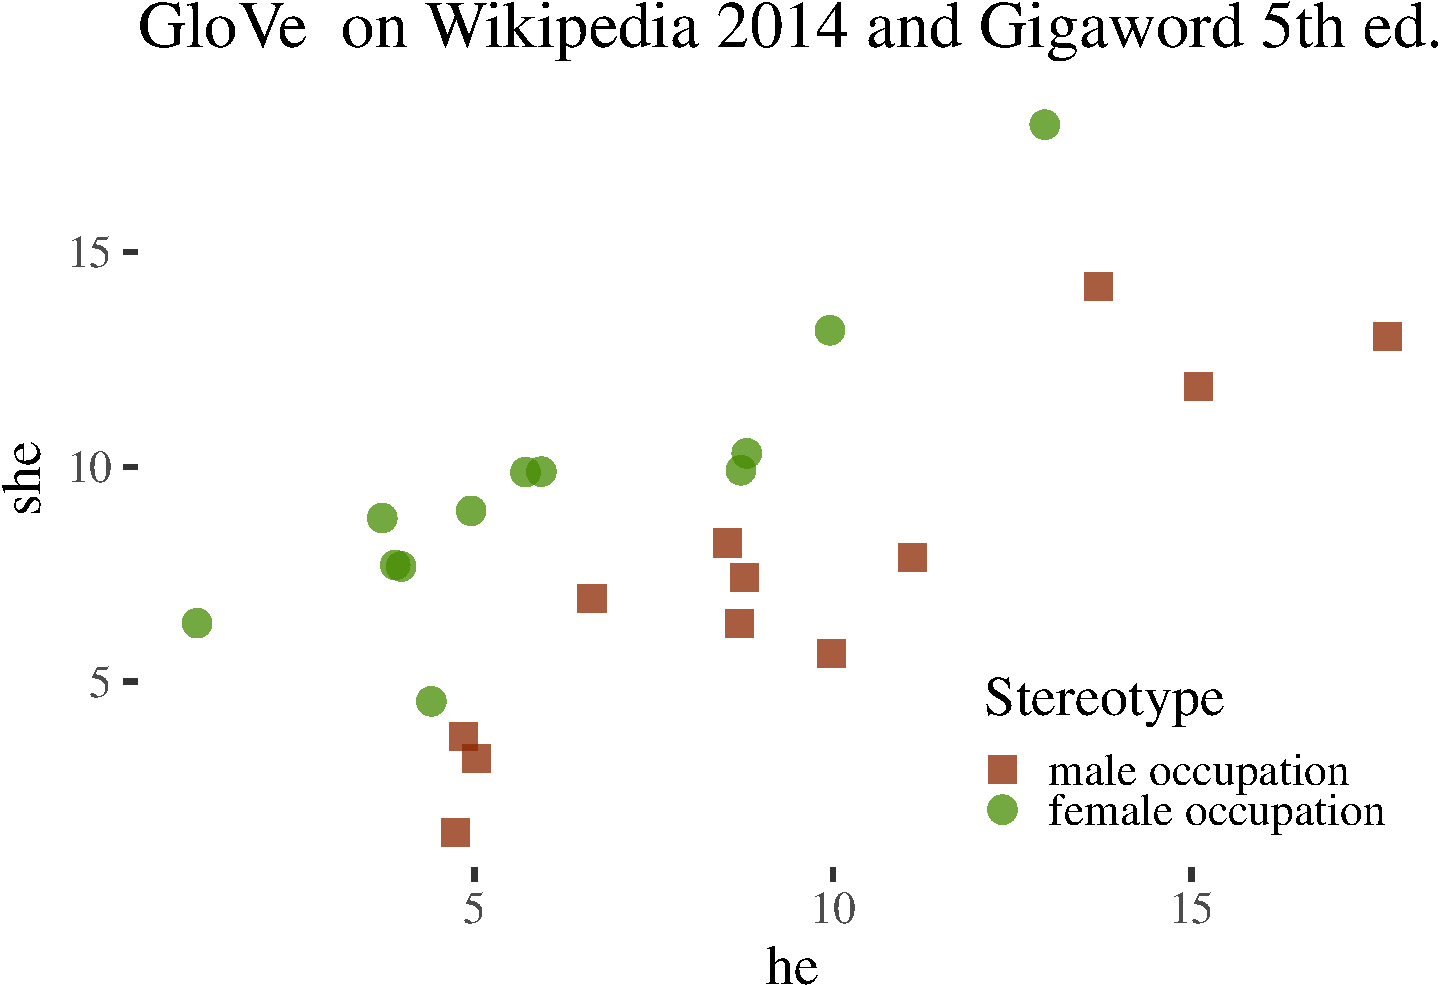
\includegraphics[width=0.6\linewidth]{presentationESSLLI_files/figure-beamer/unnamed-chunk-1-1} \end{center}

\normalsize

\end{block}

\end{frame}

\begin{frame}{Cosine-based measures of bias}

\begin{block}{Example: direct bias}

\begin{itemize}
\tightlist
\item
  The gender bias of a word \(w\) is its projection on the gender
  direction
  \(\vec{w} \cdot (\overrightarrow{he} - \overrightarrow{she})\)
\end{itemize}

\begin{itemize}
\tightlist
\item
  Given the (ideally) gender neutral words \(N\) and the gender
  direction \(g\) the direct gender bias is: 
\end{itemize}

\vspace{-2mm}

\begin{align}
\mathsf{directBias_c(N,g)} & = \frac{\sum_{w\in N}\vert \mathsf{cos}(\vec{w},g)\vert^c}{\vert N \vert }
\end{align}

\footnotesize 

(Bolukbasi, Chang, Zou, Saligrama, \& Kalai,
\protect\hyperlink{ref-Bolukbasi2016Man}{2016})

\end{block}

\end{frame}

\begin{frame}{Cosine-based measures of bias}

\begin{block}{Example: Word Embedding Association Test (WEAT)}

\begin{align*}
s(t,A,B) & = \frac{\sum_{a\in A}f(t,a)}{\vert A\vert} - \frac{\sum_{b\in B}f(t,b)}{\vert B\vert}
\\
WEAT(A,B) & = \frac{
\mu\left(\{s(x,A,B)\}_{x\in X}\right) -\mu\left(\{s(y,A,B)\}_{y\in Y}\right) 
}{
\sigma\left(\{s(w,A,B)\}_{w\in X\cup Y}\right)
}
\end{align*}

\begin{itemize}
\item
  \(t\) is a term, \(A, B\) are sets of stereotype attribute words, \$X,
  \(Y\) are protected group words
\item
  For instance, \(X\) might be a set of male names, \(Y\) a set of
  female names, \(A\) might contain stereotypically male-related career
  words, and \(B\) stereotypically female-related family words
\item
  \(s\)-values are used as datapoints in statistical significance tests
\end{itemize}

\footnotesize

(Caliskan, Bryson, \& Narayanan,
\protect\hyperlink{ref-Caliskan2017semanticsBiases}{2017}) with
extensions in (Lauscher \& Glavas,
\protect\hyperlink{ref-Lauscher2019multidimensional}{2019}) and
applications in (Garg, Schiebinger, Jurafsky, \& Zou,
\protect\hyperlink{ref-Garg2018years}{2018})

\end{block}

\end{frame}

\begin{frame}{Cosine-based measures of bias}

\begin{block}{Our main target: Mean Average Cosine Similarity (MAC)}

\begin{align*}
S(t_i, A_j) & = \frac{1}{\vert A_j\vert}\sum_{a\in A_j}\mathsf{cos}(t,a) \\
MAC(T,A) & = \frac{1}{\vert T \vert \,\vert A\vert}\sum_{t_i \in T }\sum_{A_j \in A} S(t_i,A_j)
\end{align*}

\begin{itemize}
\item
  \(T = \{t_1, \dots, t_k\}\) is a class of protected words
\item
  each \(A_j\in A\) is a set of attributes stereotypically associated
  with a protected word
\end{itemize}

\begin{itemize}
\tightlist
\item
  The t-tests they employ are run on average cosines used to calculate
  MAC
\end{itemize}

\footnotesize 

(Manzini, Lim, Tsvetkov, \& Black,
\protect\hyperlink{ref-Manzini2019blackToCriminal}{2019})

\end{block}

\end{frame}

\begin{frame}{Cosine-based measures of bias}

\begin{block}{Our main target: Mean Average Cosine Similarity (MAC)}

\footnotesize 

\begin{table}

\caption{\label{tab:religionTableHeadEarly}Rows the religion dataset.}
\centering
\resizebox{\linewidth}{!}{
\begin{tabular}[t]{llrr}
\toprule
protectedWord & wordToCompare & cosineDistance & cosineSimilarity\\
\midrule
jew & greedy & 0.6947042 & 0.3052958\\
rabbi & greedy & 1.0306175 & -0.0306175\\
rabbi & conservative & 0.7175887 & 0.2824113\\
christian & uneducated & 0.5081939 & 0.4918061\\
christianity & cheap & 1.2816164 & -0.2816164\\
muslim & terrorist & 0.2726106 & 0.7273894\\
\bottomrule
\end{tabular}}
\end{table}

\normalsize

\end{block}

\end{frame}

\begin{frame}{Cosine-based measures of bias}

\begin{block}{Known challenges}

\begin{itemize}
\item
  Gender-direction might be an indicator of bias, but is insufficient.
  After debiasing other non-gendered words can remain in biased
  relations (Gonen \& Goldberg,
  \protect\hyperlink{ref-Gonen2019lipstick}{2019})
\item
  Methods which involve analogies and their evaluations by human users
  on Mechanical Turk are unreliable (Nissim, Noord, \& Goot,
  \protect\hyperlink{ref-Nissim2020fair}{2020})
\end{itemize}

\end{block}

\end{frame}

\begin{frame}{Some methodological problems}

\begin{block}{Word list choice is unprincipled}

We run with it for comparison

\pause

\end{block}

\begin{block}{No design considerations to sample size}

We investigate the uncertainty that arises from raw sample sizes

\end{block}

\end{frame}

\begin{frame}{Some methodological problems}

\begin{block}{No word class distinction and no control group}

We make the subclasses clear, add human neutral predicates and neutral
predicates for control

\footnotesize 

\begin{table}

\caption{\label{tab:religionTableHeadLate}Rows from extended religion dataset.}
\centering
\resizebox{\linewidth}{!}{
\begin{tabular}[t]{lllrrl}
\toprule
protectedWord & wordToCompare & wordClass & cosineDistance & cosineSimilarity & connection\\
\midrule
torah & hairy & jewish & 1.170 & -0.170 & associated\\
christian & dirty & muslim & 0.949 & 0.051 & different\\
judaism & cheap & jewish & 1.232 & -0.232 & associated\\
christianity & familial & christian & 0.645 & 0.355 & associated\\
mosque & approve & neutral & 0.995 & 0.005 & none\\
imam & carry & human & 0.993 & 0.007 & human\\
mosque & merging & neutral & 0.868 & 0.132 & none\\
muslim & nationalized & neutral & 0.870 & 0.130 & none\\
\bottomrule
\end{tabular}}
\end{table}

\normalsize

\end{block}

\end{frame}

\begin{frame}{Some methodological problems}

\begin{block}{Outliers and surprisingly dissimilar words}

We study those by visualizations and uncertainty estimates

\pause

\end{block}

\begin{block}{No principled interpretation}

\begin{longtable}[]{@{}ll@{}}
\toprule
Religion Debiasing & MAC (distance)\tabularnewline
\midrule
\endhead
Biased & 0.859\tabularnewline
Hard Debiased & 0.934\tabularnewline
Soft Debiased (\(\lambda\) = 0.2) & 0.894\tabularnewline
\bottomrule
\end{longtable}

What values are sufficient for the presence of bias and what differences
are sign of real improvement? Low \(p\)-values are not high effect
indicators!

We compare HPDIs.

\end{block}

\end{frame}

\begin{frame}{The problem with pre-averaging}

\end{frame}

\begin{frame}{Bayesian estimation}

\begin{center}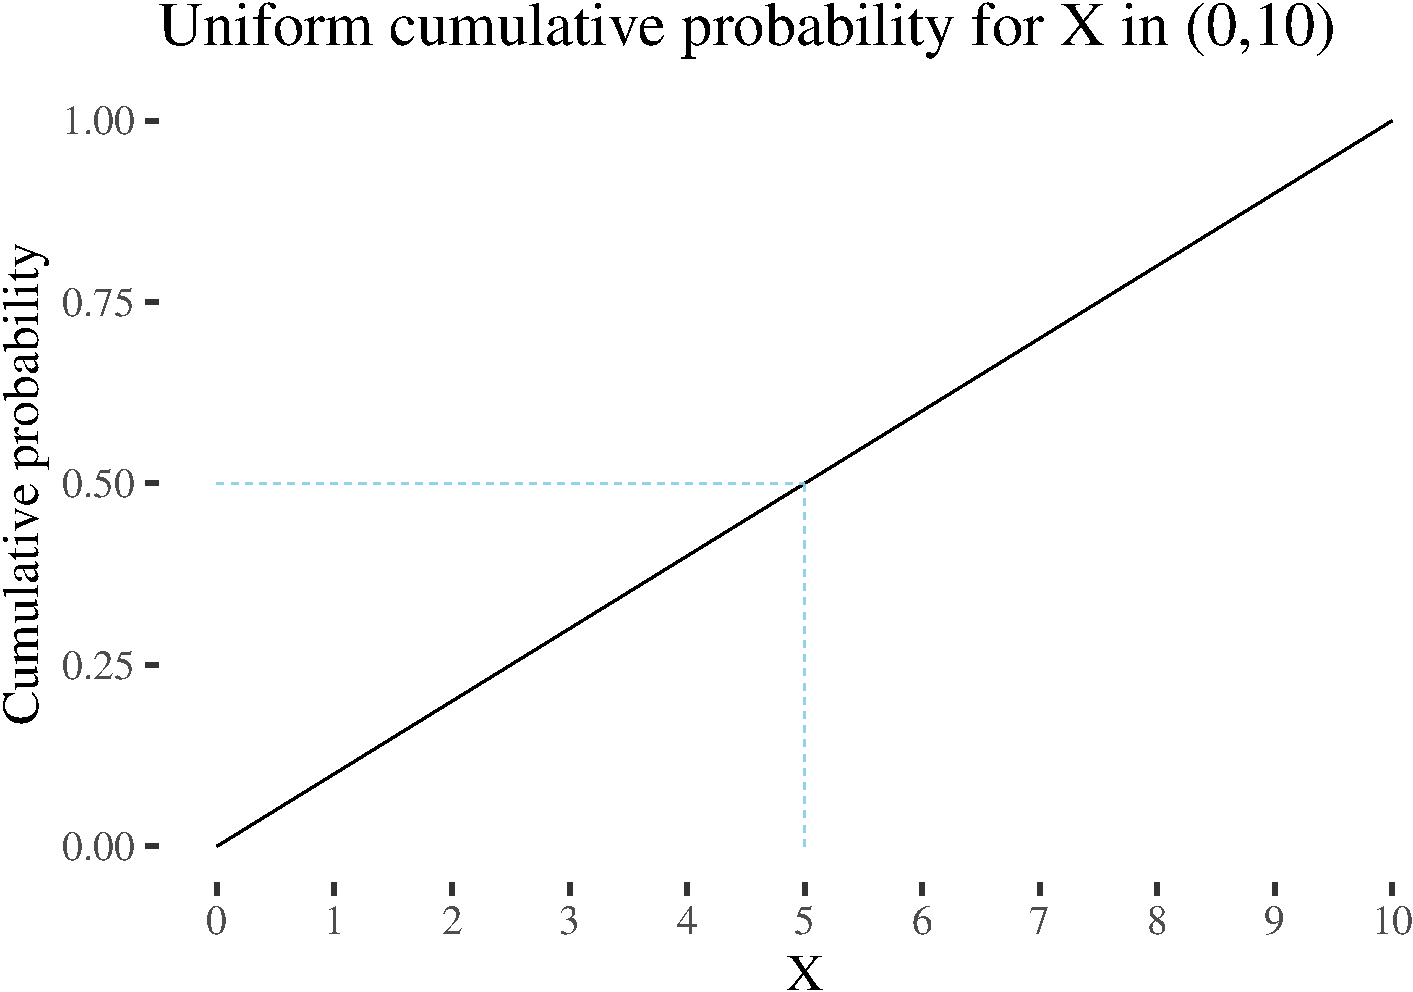
\includegraphics[width=1.05\linewidth]{presentationESSLLI_files/figure-beamer/unnamed-chunk-2-1} \end{center}

\end{frame}

\begin{frame}{Bayesian estimation}

\begin{center}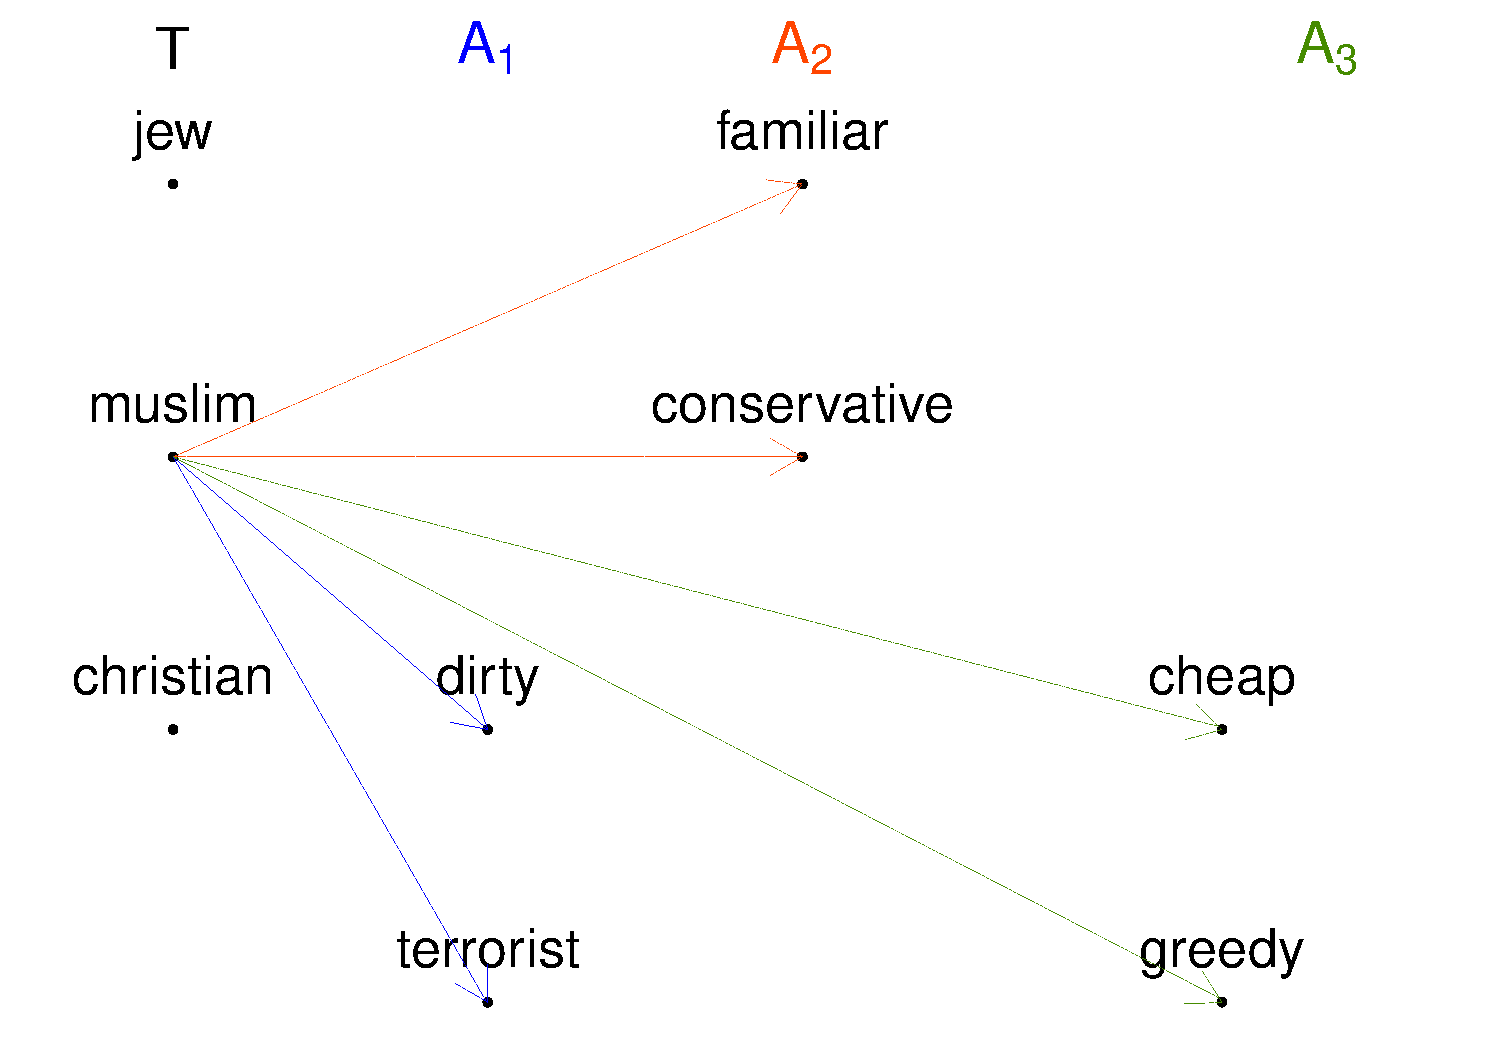
\includegraphics[width=1.05\linewidth]{presentationESSLLI_files/figure-beamer/unnamed-chunk-3-1} \end{center}

\end{frame}

\begin{frame}{Effects of debiasing}

\begin{block}{Further work}

\begin{itemize}
\tightlist
\item
  downstream tasks
\end{itemize}

\end{block}

\end{frame}

\begin{frame}{References}

\tiny

\hypertarget{refs}{}
\hypertarget{ref-Bolukbasi2016Man}{}
Bolukbasi, T., Chang, K., Zou, J. Y., Saligrama, V., \& Kalai, A.
(2016). Man is to computer programmer as woman is to homemaker?
Debiasing word embeddings. \emph{CoRR}, \emph{abs/1607.06520}. Retrieved
from \url{http://arxiv.org/abs/1607.06520}

\hypertarget{ref-Caliskan2017semanticsBiases}{}
Caliskan, A., Bryson, J. J., \& Narayanan, A. (2017). Semantics derived
automatically from language corpora contain human-like biases.
\emph{Science}, \emph{356}(6334), 183--186.
\url{https://doi.org/10.1126/science.aal4230}

\hypertarget{ref-Garg2018years}{}
Garg, N., Schiebinger, L., Jurafsky, D., \& Zou, J. (2018). Word
embeddings quantify 100 years of gender and ethnic stereotypes.
\emph{Proceedings of the National Academy of Sciences}, \emph{115}(16),
E3635--E3644. \url{https://doi.org/10.1073/pnas.1720347115}

\hypertarget{ref-Gonen2019lipstick}{}
Gonen, H., \& Goldberg, Y. (2019). Lipstick on a pig: Debiasing methods
cover up systematic gender biases in word embeddings but do not remove
them. \emph{Proceedings of the 2019 Conference of the North American
Chapter of the Association for Computational Linguistics: Human Language
Technologies, Volume 1 (Long and Short Papers)}, 609--614. Minneapolis,
Minnesota: Association for Computational Linguistics.
\url{https://doi.org/10.18653/v1/N19-1061}

\hypertarget{ref-Lauscher2019multidimensional}{}
Lauscher, A., \& Glavas, G. (2019). Are we consistently biased?
Multidimensional analysis of biases in distributional word vectors.
\emph{CoRR}, \emph{abs/1904.11783}. Retrieved from
\url{http://arxiv.org/abs/1904.11783}

\hypertarget{ref-Manzini2019blackToCriminal}{}
Manzini, T., Lim, Y. C., Tsvetkov, Y., \& Black, A. W. (2019).
\emph{Black is to criminal as caucasian is to police: Detecting and
removing multiclass bias in word embeddings}.

\hypertarget{ref-Nissim2020fair}{}
Nissim, M., Noord, R. van, \& Goot, R. van der. (2020). Fair is better
than sensational: Man is to doctor as woman is to doctor.
\emph{Computational Linguistics}, \emph{46}(2), 487--497.
\url{https://doi.org/10.1162/coli_a_00379}

\end{frame}

\end{document}
